\chapter{Testy środowiska symulacyjnego}
\label{sec:tests}
W tym rozdziale przedstawione są różne konfiguracje pakietów, wraz z wykresami ruchów platform, oraz wnioski płynące z tych zachowań.
Każdy test wymaga innego podłączenia pakietów do siebie nawzajem.

Wyniki pomiarów zostały zebrane za pomocą ROSowego narzędzia \texttt{rosbag}, a następnie wyeksportowane do pliku CSV. Za pomocą programu Gnuplot narysowano wykresy.

\section{Testy odometrii}
	\label{sec:test_odometry}
	Model czujnika enkoderów zwraca aktualną prędkość i pozycję kół modelu dynamiki.
	W ten sposób jest możliwe dokładniejsze określenie pozycji platformy, niż bazując na modelu kinematycznym.
	Jednakże, ta metoda także ma swoje ograniczenia, ze względu na poślizgi, zatem program sterujący nie może w pełni bazować na tych czujnikach, a jedynie powinien używać ich pomocniczo.
	
	W tym teście obliczono pozycję modelu dynamiki, bazując na danych zebranych przez modele enkoderów, skorzystano z połączenia przedstawionego na rysunku \ref{uml:encoders}.
	Platforma posiada algorytm, który wewnętrznie, korzystając z enkoderów i modelu kinematyki, oblicza pozycję, w której powinien znajdować się robot.
	
	Za pomocą pakietu nadającego sterowanie z pliku, opisanego w sekcji \ref{sec:gramofon}, podano robotowi i modelowi proste sterowanie.
	Ruch odbywał się przez 10 \si{\second} z prędkością 0,1 \si{\metre\per\second} na dystansie 1 \si{\metre}, kolejno w kierunkach -X, -Y, X i Y.
	Zmiana kierunku prędkości odbywała się natychmiastowo, powodując poślizgi.
	W tym teście nie nadawano prędkości kątowej.
	
	\begin{figure}[H]
		\centering
		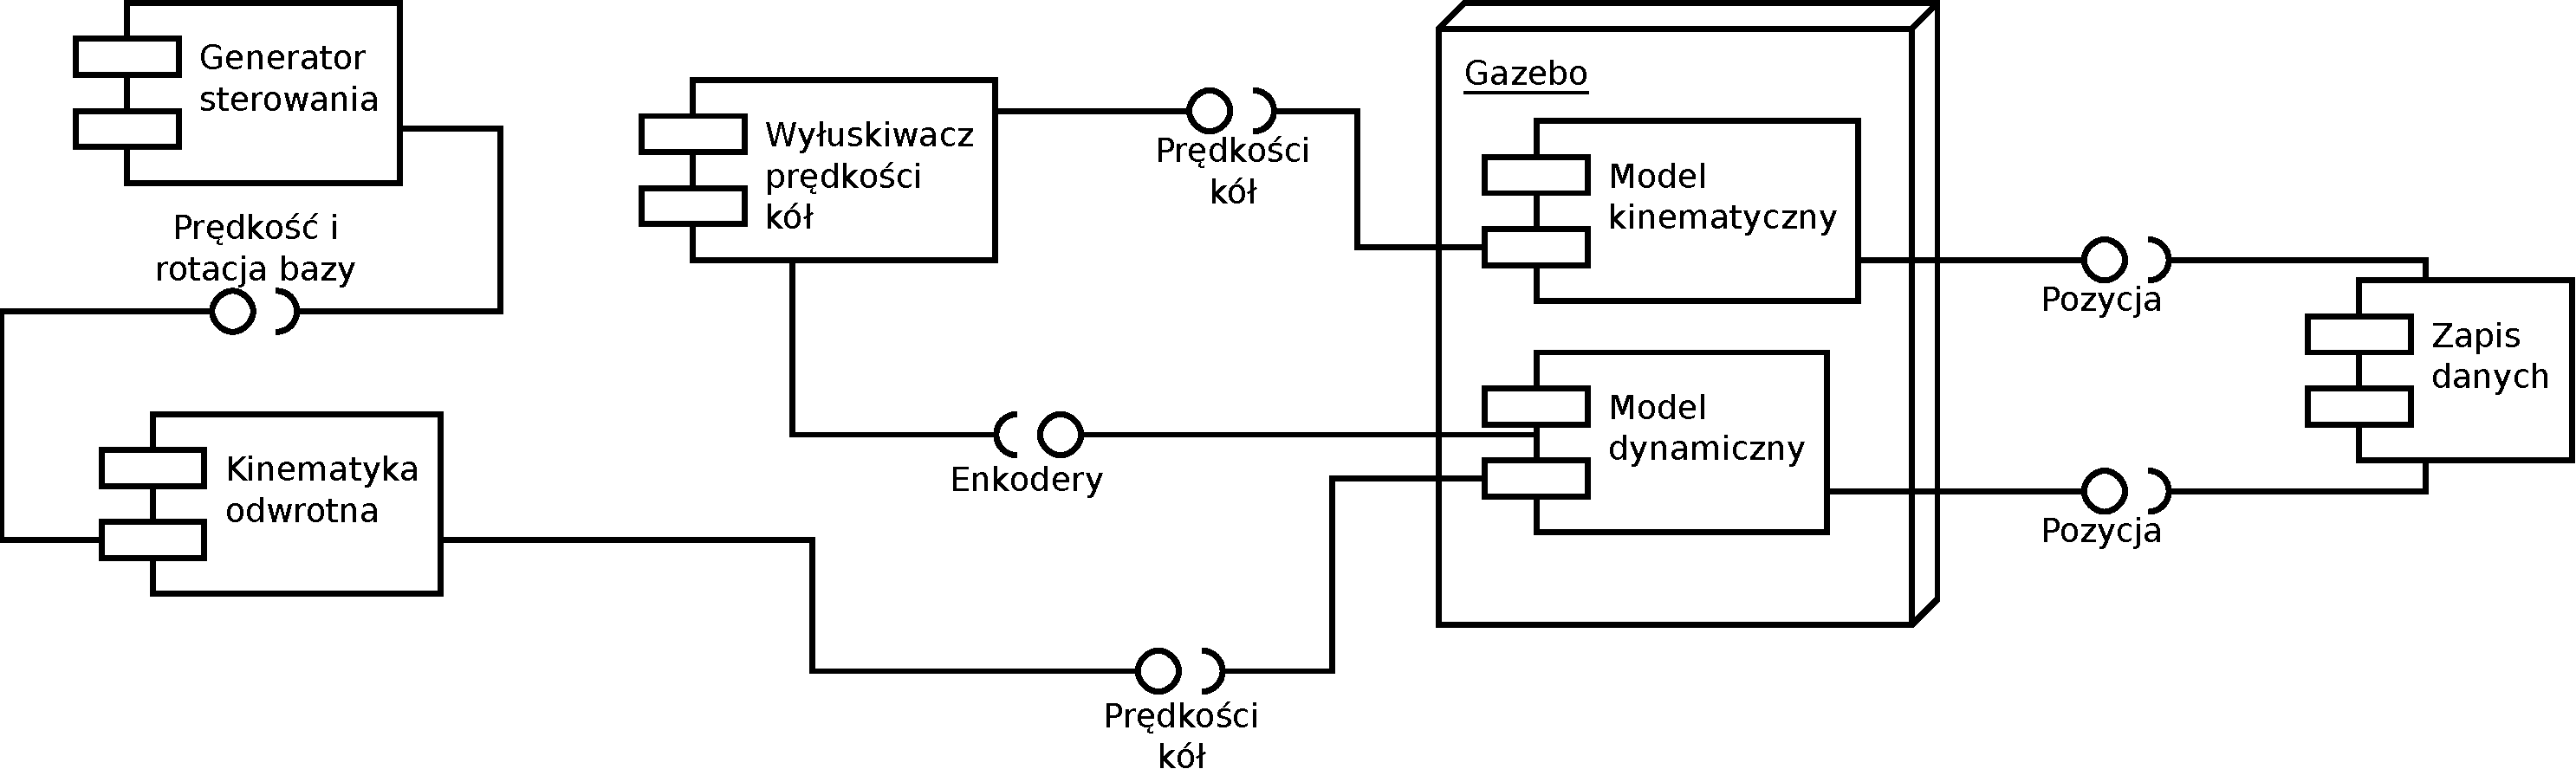
\includegraphics[width=\textwidth]{uml/encoders.pdf}
			\caption{Połączenie pakietów w celu sprawdzenia poprawności działania enkoderów modelu dynamiki.}
		\label{uml:encoders}
	\end{figure}
	
	Wyjście enkoderów modelu dynamiki wyłuskane jest z wiadomości i podane dla modelu kinematyki.
	
	\begin{figure}[H]
		\centering
		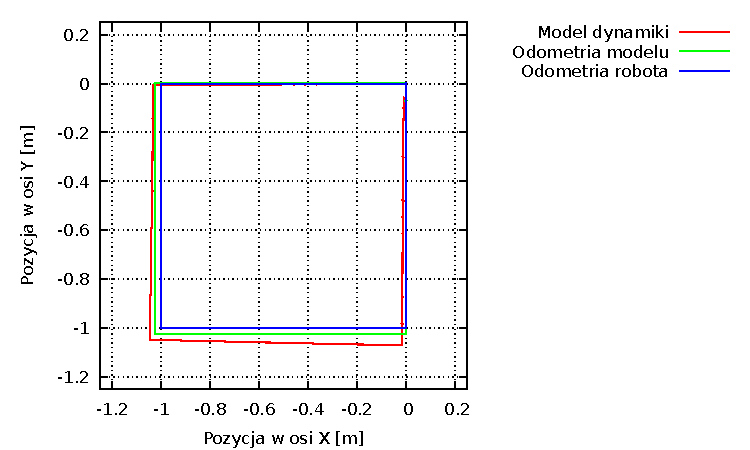
\includegraphics[width=\textwidth]{plots/odometry.pdf}
			\caption{Porównanie pozycji modelu dynamiki z pozycją platformy.}
		\label{plot:encoders}
	\end{figure}
	
	\subsubsection{Odometria robota}
		Pierwszą cechą wykresu jest to, że dane z algorytmu odometrii na robocie pokrywają się z zadaną trasą.
		Jest tak prawdopodobnie, ponieważ silniki platformy dysponują dużą mocą, a także dużym oporem.
		Potrzeba jest zatem odpowiedniej siły tarcia o podłoże w celu wymuszenia obrotu takiego koła wbrew zadanemu sterowaniu.
		To powoduje, że koło jest niepodatne na warunki zewnętrzne w większym stopniu, niż jest to modelowane.
		Zatem pozycja wyliczona z odometrii będzie się niemal pokrywać z pozycją na zadanej trasie.
		
		To nie oznacza, że wygenerowana trasa pokrywała się z rzeczywistością. Trasa obliczona na podstawie skanera laserowego znajduje się na wykresie \ref{sec:test_pose}.
		
	\subsubsection{Pozycja modelu}
		Na skutek błędów numerycznych maszyny do symulacji fizyki, symulacji nie na systemie czasu rzeczywistego, braku oporów i skomplikowanej budowy modelu, następuje
		nieprzewidywalny ruch wo kół osi Z w trakcie nagłej zmiany kierunku jazdy.
		Za każdym skrętem dodawany jest obrót kątowy wokół osi Z do orientacji modelu platformy, który jest niewykrywalny przez modele enkoderów, a zatem być może powstaje na skutek
		poślizgu.
		Dlatego też różnica pomiędzy pozycją na zadanej trasie, a pozycją modelu zwiększa się w czasie.
		
		Model także przejechał większą odległość, niż zadana. Być może jest to spowodowane sposobem liczenia kolizji w maszynie symulacyjnej fizyki, rzeczywista odległość pomiędzy osią koła i podłożem jest większa od promienia koła. Poślizg nie wpływa na to zjawisko, gdyż w testach bez nagłego hamowania nadal występuje i jest wykrywany przez model kinematyki.
		
\section{Pozycja obliczona ze skanerów laserowych}
	\label{sec:test_pose}
	Pozycja modelu została łatwo wygenerowana, ponieważ symulacja odbywała się w przestrzeni wirtualnej.
	Pozycja platformy nie mogła być łatwo określona. Posłużono się algorytmem ROSowego pakietu \texttt{laser\_scan\_matcher}, który na podstawie 
	danych z jednego i drugiego skanera laserowego i odometrii określił aktualną pozycję platformy. Określenie pozycji jest obarczone błędem wynikającym
	z błędów pomiarowych czujników, stąd obliczona trasa nie składa się z odcinków i posiada szum.
	
	To jest ten sam eksperyment co w sekcji \ref{sec:test_odometry}.
	Pakiety zostały połączone w prostszy sposób, jak na rysunku \ref{uml:test_pose}, model kinematyczny generuje trasę na podstawie zadanych prędkości.
	
	\begin{figure}[H]
		\centering
		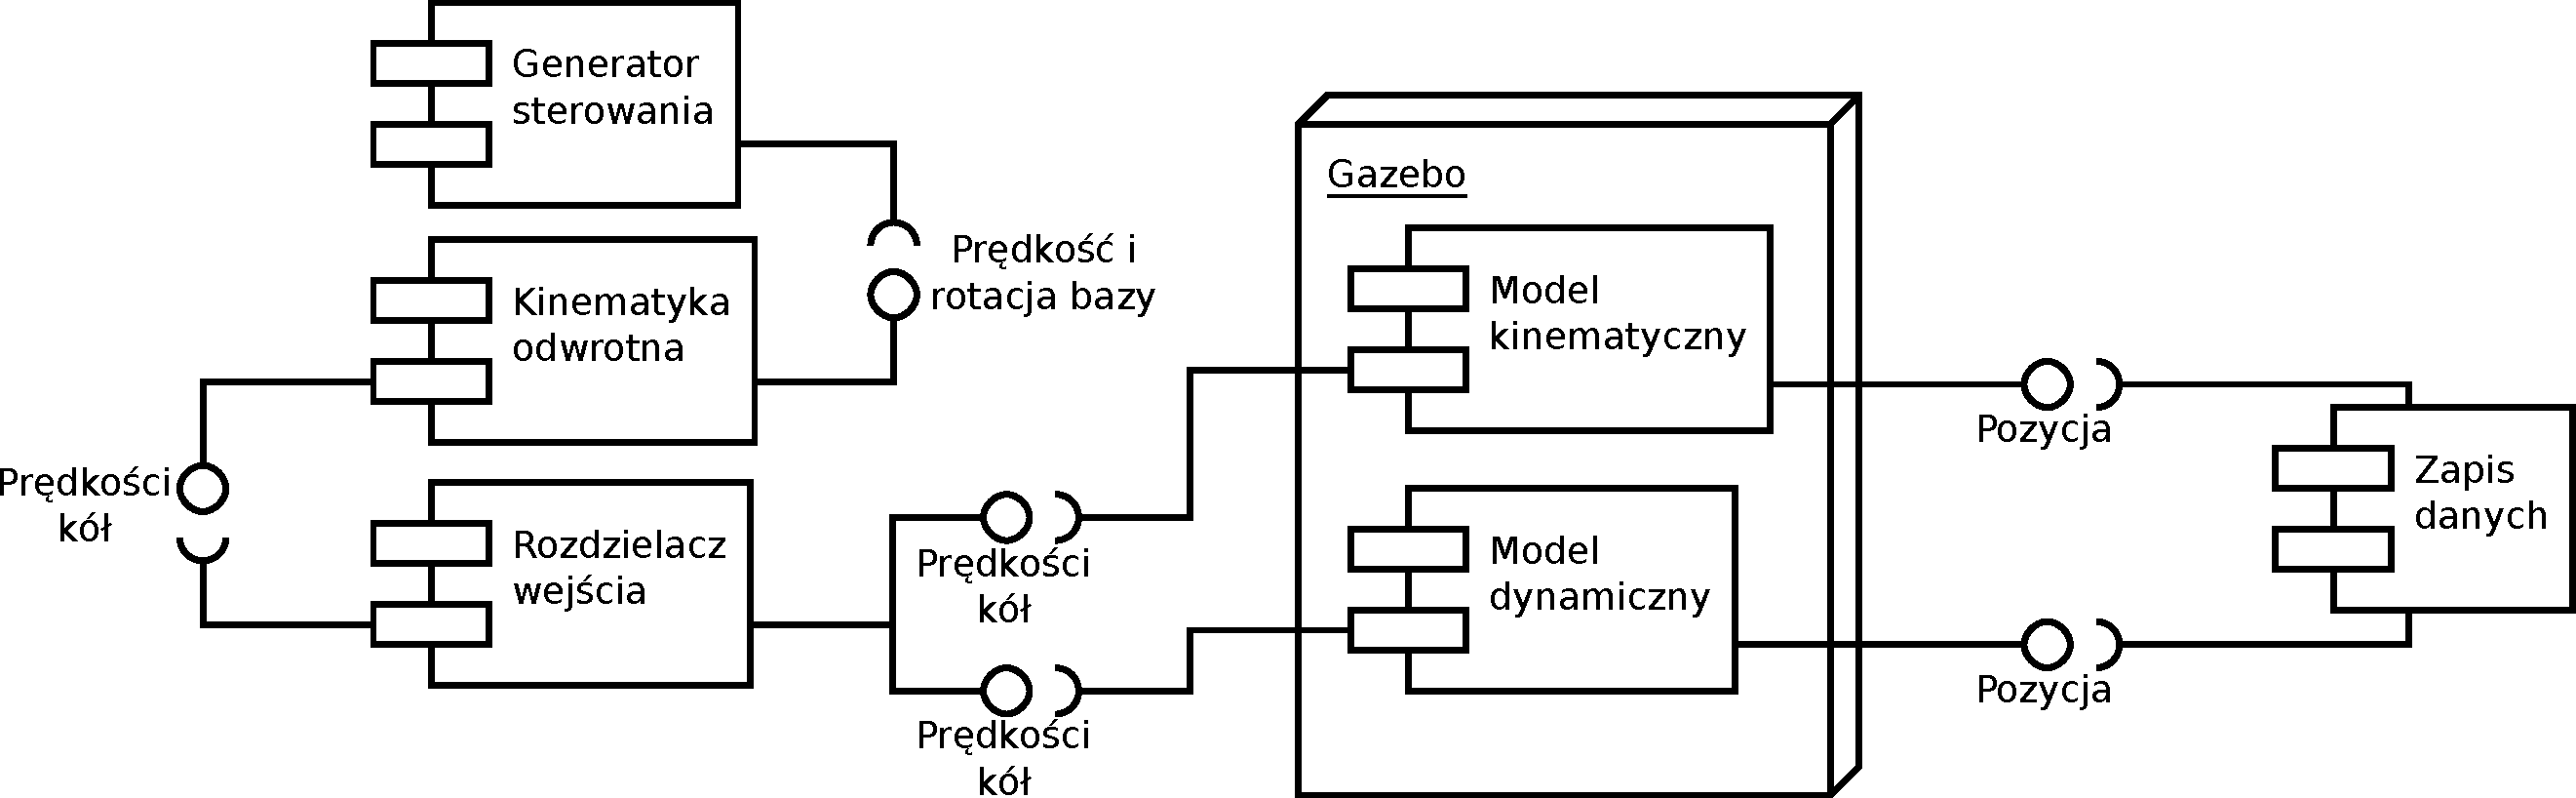
\includegraphics[width=\textwidth]{uml/gramofon.pdf}
		\caption{Połączenie pakietów dla testu pozycji modelu.}
		\label{uml:test_pose}
	\end{figure}
	
	\begin{figure}[H]
		\centering
		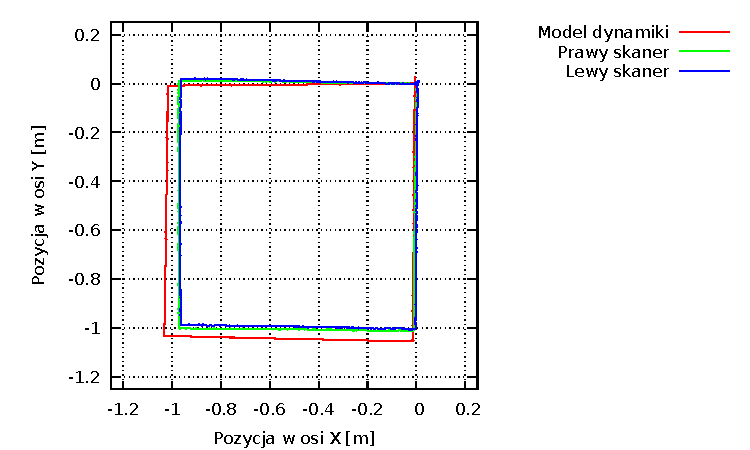
\includegraphics[width=\textwidth]{plots/matcher.pdf}
		\caption{Pozycja robota, obliczona z jednego lub drugiego skanera laserowego i model.}
		\label{plot:pose}
	\end{figure}
	
	\subsubsection{Powtarzalność jazdy modelu}
		Jak wcześniej wspomniano, poślizgi nadają modelowi nieprzewidywalne kąty w trakcie nagłej zmiany prędkości. 
		Dlatego też trasy modelu platformy w tym i wcześniejszym teście z sekcji \ref{sec:test_odometry} różnią się. 
	\subsubsection{Wyznaczenie pozycji}
		Duże podobieństwo pozycji wyznaczonej przez jeden i drugi skaner wskazuje, że algorytm działa dobrze i daje przewidywalne wyniki.
		Trasa przejazdu również jest prawdopodobna.
	\subsubsection{Trasa robota}
		Robot jadąc równolegle do osi X, jechał w bok i pokonał krótszą trasę niż przy jeździe równolegle do osi Y. Jak wspomniano w sekcji \ref{sec:robot_movement}, powodowało to większy obrót rolek
		niż przy jeździe na wprost, co powodowało większy opór ruchu i w efekcie przejazd wolniej od zadanej prędkości i po krótszej trasie.
		Model nie jest podany na tę właściwość, gdyż kule, symulujące koła, są symetryczne.
	
\section{Ruch obrotowy}
	\label{sec:test_rotation}
	W tym teście pakiety zostały podłączone tak samo, jak wcześniej, według wykresu \ref{uml:test_pose}.
	
	Test polegał na jeździe w bok z prędkością 0,1 \si{\metre\per\second}, tak samo jak w poprzednim teście, następnie obrocie wokół osi Z o 90° przez 10 \si{\second} z prędkością $\frac{\pi}{20}$ \si{\radian\per\second} i ponownej jeździe w bok. Tak 4 razy, dla każdego boku kwadratu.
	Pozycja robota została wyznaczona z czujników laserowych i odometrii w taki sam sposób, jak w teście \ref{sec:test_pose}.
	
	\begin{figure}[H]
		\centering
		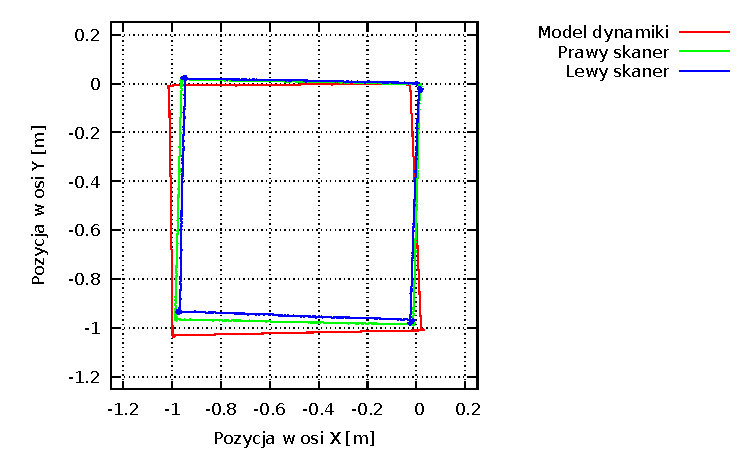
\includegraphics[width=\textwidth]{plots/rotation_matcher.pdf}
		\caption{Pozycja robota, obliczona z jednego lub drugiego skanera laserowego i model.}
		\label{plot:rotation}
	\end{figure}
	
	\subsubsection{Trasa robota}
		Na początku eksperymentu nastąpił poślizg, który obrócił platformę o nieznaczny kąt.
		Przez to trasa jest obrócona względem zaplanowanej.
	\subsubsection{Trasa modelu}
		Właściwość modelu powodująca, że pokonuje większą trasę, niż zadana objawia się także w trakcie obrotu, gdzie wykonuje większy kąt niż prosty.
		Dlatego kolejne segmenty trasy są coraz mniej równoległe do osi układu współrzędnych.
		Na kątach widać także, że model nie obraca się wokół swojego środka (początku lokalnego układu współrzędnych), tylko od lekko przesuniętego w bok
		punktu ciężkości. Pomimo, że wartości ogniw zostały dobrane symetrycznie, jak widać nie wszystkie wartości się równoważą.
		Jest to cecha charakterystyczna dla maszyn symulacji fizyki w czasie rzeczywistym.
		
\section{Jednostka inercyjna}
\label{sec:test_imu}
	\begin{figure}[H]
		\centering
		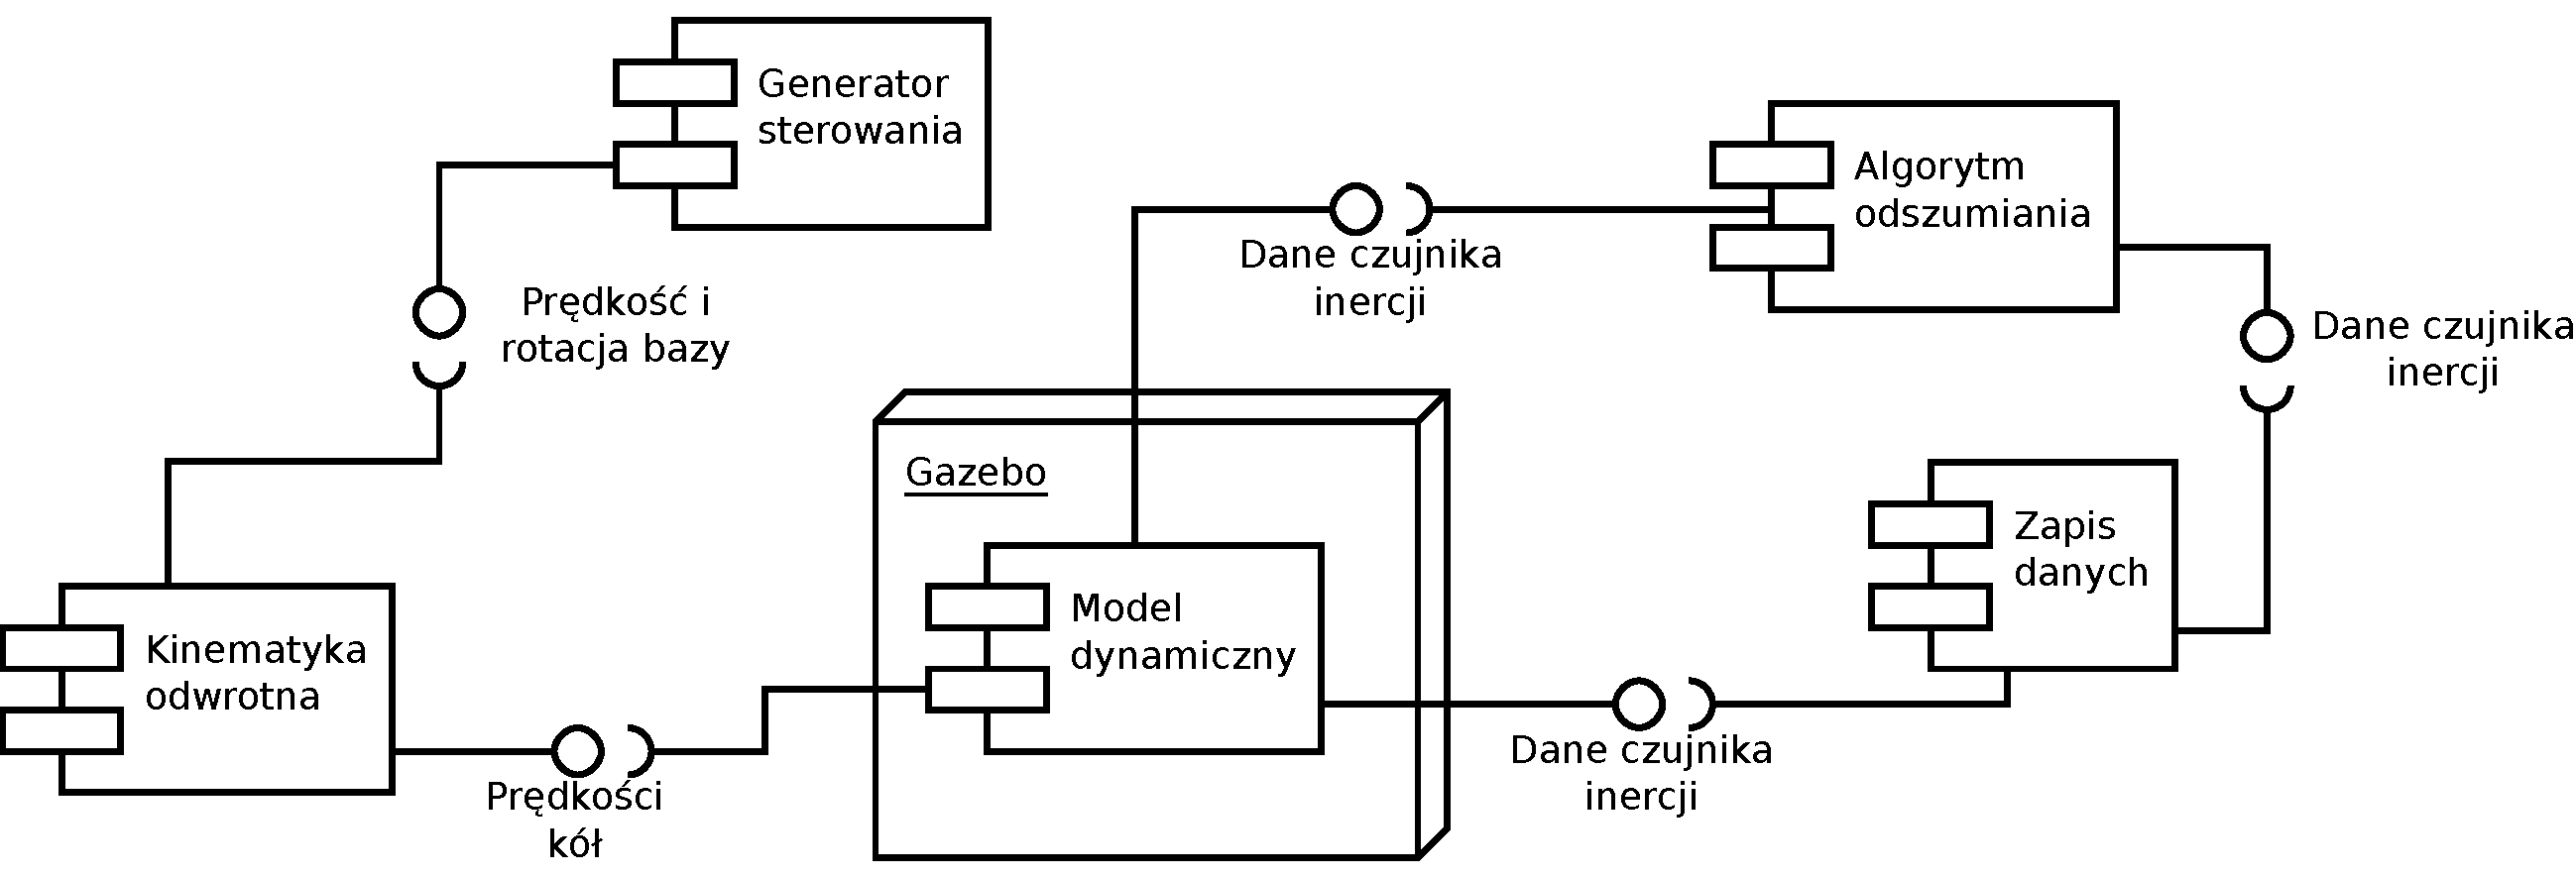
\includegraphics[width=\textwidth]{uml/wewucho.pdf}
		\caption{Połączenie pakietów dla testu jednostki inercyjnej.}
		\label{uml:test_imu}
	\end{figure}
	\subsection{Akcelerometr}
		Dane zostały zebrane w trakcie testu \ref{sec:test_pose}.
		Połączenie pakietów w sposób pokazany na rysunku \ref{uml:test_imu}.
		Dane wygenerowane przez ten czujnik są obarczone bardzo dużym błędem.
		
		\begin{figure}[H]
			\centering
			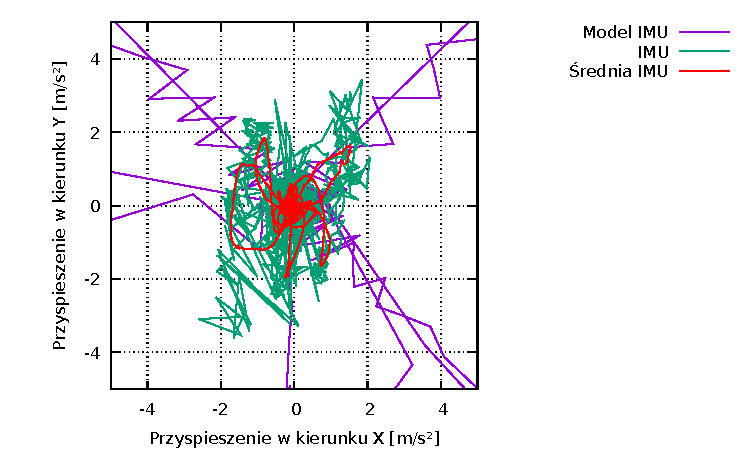
\includegraphics[width=\textwidth]{plots/wewucho.pdf}
			\caption{Odczyt akcelerometra z jednostki inercyjnej i jej modelu.}
			\label{plot:imu}
		\end{figure}
		
		\subsubsection{Impulsy na wykresie modelu}
			W trakcie testu następowały kolejne przyspieszenia i opóźnienia bazy w zadanych kierunkach, to widać jako impulsy na wykresie.
			Na początku platforma zaczęła poruszać się w kierunku -X i w tą stronę zostało nadane pierwsze przyspieszenie.
			Nie jest znana jego wielkość, gdyż było to wysłanie jednej wiadomości, bez płynnego narastania prędkości.
			
			Następnie zadziałało przyspieszenie zmieniające prędkość liniową platformy o 90°, co oznacza że impuls jest obrócony o 45° względem układu współrzędnych.
			Impuls wystąpił w kierunku (X,-Y). 
			
			Podobna zmiana prędkości nastąpiła jeszcze dwa razy, generując kolejne, symetryczne impulsy.
			
			Platforma zatrzymała się, generując opóźnienie w kierunku -Y, co także widać na wykresie.
			
			Przeprowadzanie podobnych testów pokazuje, że nawet jeśli ustawić zaplanowane przyspieszenie modelu, to i tak czujnik nie zwraca poprawnych amplitud.
			Jedyne, co wiadomo to to, że generuje proporcjonalnie większe wartości dla większych przyspieszeń.
			Również istnieje korelacja pomiędzy osiami, na przykład natychmiastowe zatrzymanie się w jednym z kierunków powoduje inne przyspieszenie, niż w innym kierunku.
			Co zresztą jest logiczne, gdyż osie kół stawiają większy opór, gdy działający na nie moment siły jest skierowany prostopadle do osi, niż równolegle. 
			Zatem większe opóźnienie będzie przy hamowaniu z jazdy w bok, niż jazdy w przód.
			
			Szum spowodowany jest potrzebą różniczkowania prędkości obliczanej dyskretnie. Wartości mas i momentów inercji ogniw modelu mocno wpływają na kształt, kolerację
			osi i szum na wykresie. Nie jest technologicznie możliwe zamodelować doskonałej jednostki inercyjnej ze względu na błędy numeryczne, algorytmy użyte w maszynie
			symulującej fizykę i system operacyjny na którym pracuje symulator.
			
		\subsubsection{Wykres czujnika}
			Porównując te dwa wykresy razem, nie widać zależności, jednak zastosowanie prostego uśrednienia powoduje, że impulsy wygenerowane przez robota również są widoczne.
			Aby użyć tego czujnika do obliczania pozycji, trzeba wpierw użyć zaawansowanego algorytmu odszumiającego i wyprowadzić eksperymentalnie zależności pomiędzy czujnikami
			osi (macierz kowariancji).
			Dopiero wtedy można wprowadzić dodatkowy szum do modelu jednostki inercyjnej w celu przybliżenia jej wyjścia do rzeczywistego urządzenia.

			
\subsection{Żyroskop}
		\label{sec:test_ang}
		Czujnik prędkości kątowej korzysta z żyroskopu i zwraca prędkość kątową we wszystkich trzech osiach.
		Ponieważ jednak platforma porusza się po płaskim terenie, wymagany jest jedynie czujnik mierzący obrót wokół osi Z, czyli w górę.
		Drugą osią wykresu może być zatem czas nadania pakietu. Te dane zostały zebrane w trakcie testu \ref{sec:test_pose}.
		
		\begin{figure}[H]
			\centering
			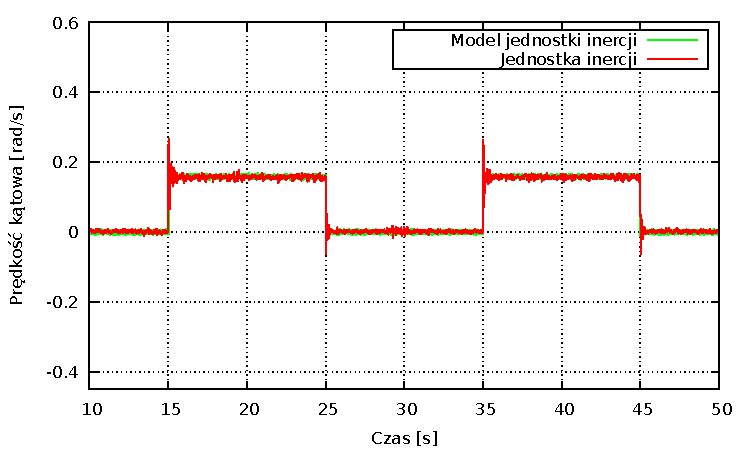
\includegraphics[width=\textwidth]{plots/wewucho_ang.pdf}
			\caption{Odczyt żyroskopu z jednostki inercyjnej i jej modelu.}
			\label{plot:ang}
		\end{figure}
		
		Ponieważ maszyna do symulacji fizyki wewnętrznie posiada informację o prędkościach obiektów, model tego czujnika po prostu zwraca gotowe dane. 
		To powoduje, że praktycznie pozbawiony jest szumu. 
		Aby zatem polepszyć jakość symulacji, dodano sztuczny szum do generowanych danych, zgodnie z tabelą \ref{tab:imu_noise}.
		W ten sposób wykresy są do siebie bardziej zbliżone.
		
		Jednak niektórych własności czujnika nie da się zamodelować tak łatwo. Po pierwsze, szum czujnika nie do końca ma rozkład normalny.
		Z wykresu można zobaczyć, że dane prawdopodobnie korelują z częstotliwościami obrotu kół.
		Dodatkowo, nagła zmiana prędkości kątowej powoduje zauważalny skok na wykresie, co w symulatorze jest znacznie mniej widoczne.
		Ta cecha wykresu zależy od ustawień mas i inercji ogniw modelu, lecz z kolei inne ustawienia inercji powodują większe błędy przy poruszaniu się platformy.
		
		
		
	
	
